\chapter{Funzioni: Creiamo un Linguaggio Comune}
In questo breve capitolo faremo un ripasso sulle funzioni, il quale ci permetterà di fissare un linguaggio comune per non fare confusione. Questo sarà fondamentale per dare la definizione di Variabile Aleatoria.\\
\\
Consideriamo $\Omega$ come dominio, ed $\mathcal{F}$ il codominio. Allora possiamo definire una funzione $X$:
\begin{align*}
    X:\Omega&\longrightarrow \mathcal{F}\\
    w\in\Omega &\longmapsto X(w) = x\in \mathcal{F}
\end{align*}
\begin{figure}[H]
    \centering
    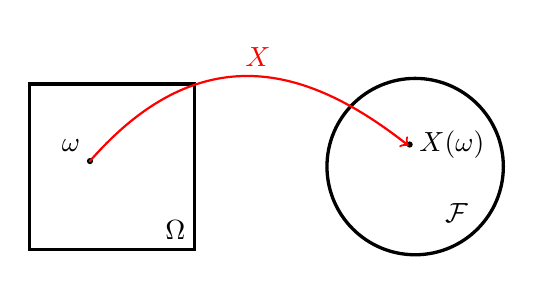
\begin{tikzpicture}[x=1cm,y=1cm,line cap=round, scale = 0.7]
  % --- Sorgente: spazio campionario Omega ---
  \draw[very thick] (0,0) rectangle (3,3);
  \node at (2.65,0.35) {$\Omega$};
  \fill (1.1,1.6) circle (1.6pt) node[above left] {$\omega$};

  % --- Bersaglio: spazio dei valori / misura ---
  \draw[very thick] (7,1.5) circle (1.6cm);
  \node at (7.75,0.65) {$\mathcal{F}$};
  \fill (6.9,1.9) circle (1.6pt) node[right] {$X(\omega)$};

  % --- Freccia curva X: Omega -> F ---
  \draw[red,thick,->]
    (1.1,1.6) .. controls (3.2,4.0) and (5.2,3.2)
    .. node[midway,above,text=red] {$X$} (6.88,1.88);
\end{tikzpicture}
\end{figure}
\noindent Avremo quindi che l'\textit{immagine di A} è definita come:
\[
    X(A) = \set{x\in\mathcal{F}\mid \exists\;\omega\in A:\;x = X(w)}\subseteq\mathcal{F}
\]
e la \textit{controimmagine} come:
\[X^{-1}(B) = \set{w\in\Omega \mid X(w)\in B}\subseteq\Omega\]
Possiamo anche considerare la classe di tutte le possibili immagini e controimmagini:
\begin{align*}
    & \set{X(A) \mid A\subseteq\Omega}\subseteq \mathcal{P}(\mathcal{F})\\
    & \set{X^{-1}(B)\mid B\subseteq \mathcal{F}}\subseteq \mathcal{P}(\Omega)
\end{align*}

\noindent Già a questo punto ci accorgiamo di una caratteristica importante: $X(\Omega)\subseteq \mathcal{F}$, ma $X^{-1}(\mathcal{F}) = \Omega$. Capiamo quindi che avremo delle proprietà ``migliori'' lavorando con la controimmagine, in quanto la controimmagine del codominio restituisce tutto lo spazio $\Omega$.

\begin{esempio}
    Partiamo da un esempio banale, ma che ci permette di iniziare a metabolizzare un linguaggio che può sembrare poco intuitivo.\\
    Sia $\Omega= \mathbb{R}=\mathcal{F}$, e consideriamo $X:\mathbb{R}\to \mathbb{R}$, tale che $\;X(w) = w^2$

    \begin{figure}[H]
        \centering
        % preambolo: \usetikzlibrary{decorations.pathreplacing,arrows.meta}
\begin{tikzpicture}[x=2cm,y=2cm, line cap=round, >=Stealth]

  %--- assi
  \draw[->] (-1.2,0) -- (2.2,0) node[right] {$\omega$};
  \draw[->] (0,-0.25) -- (0,1.5);

  % tacche e label 0 e 1
  \node[below] at (-0.12,0) {$0$};
  \draw (1,0.06)--(1,-0.06) node[below=2pt] {$1$};
  \draw (0.06,1)--(-0.06,1) node[right=10pt] {$1$};

  %--- parabola X(w) = w^2
  \draw[red,very thick,domain=-1.1:1.1,smooth,variable=\w]
    plot ({\w},{\w*\w});
  \node[red,anchor=west] at (1.1,1) {$X(\omega)=\omega^{2}$};

  %--- graffa verticale B (fino a y=1)
  \draw[decorate,decoration={brace,amplitude=6pt}, black]
    (-0.14,0.1) -- (-0.14,0.98);
  \node[black] at (-0.4,0.55) {\Large $B$};

  %--- graffa orizzontale A (da 0 a 1)
  \draw[decorate,decoration={brace,amplitude=6pt,mirror}, black]
    (0.05,-0.12) -- (0.95,-0.12);
  \node[black] at (0.5,-0.35) {\Large $A$};
    \end{tikzpicture} 
    \end{figure}
    Possiamo notare alcune cose:
    \begin{enumerate}
        \item $X(\Omega) = X(\mathbb{R}) = \mathbb{R}^+\neq\mathbb{R}$
        \item $A\subseteq\Omega, \;A = (0,1)\quad \Rightarrow\quad X((0, 1))= (0, 1)$\\
        $B\subseteq\mathcal{F}=\mathbb{R}, \;B=(0, 1) \quad \Rightarrow\quad X^{-1}((0, 1))= (-1, 0)\cup(0, 1)$
        \item $A^c = (0, 1)^c=(-\infty, 0]\cup[1, +\infty)$\\ $\Rightarrow\quad X(A^c)=[0, +\infty)$, tuttavia $(X(A))^c\quad \Rightarrow X(A^c)\neq (X(A))^c$
        \item $B = (0, 1)\subseteq\mathcal{F}\quad \Rightarrow\quad B^c = (-\infty, 0]\cup[1, +\infty)$\\
        Allora avremo che: 
        \begin{itemize}
            \item \(X^{-1}(B^c) = (-\infty, -1]\cup\{0\}\cup[1, +\infty)\)
            \item \((X^{-1}(B))^c = (-\infty, -1]\cup\{0\}\cup[1, +\infty)\)
        \end{itemize}
        $\Rightarrow\quad X^{-1}(B^c) = (X^{-1}(B))^c\;$, ossia che le operazioni commutano!
        \item $C = (-1, 0)\subseteq\mathcal{F};\quad B\cap C= (0, 1)\cap(-1, 0) = \varnothing$, dove:
        \begin{itemize}
            \item $X^{-1}(B\cap C) = \varnothing$
            \item $X^{-1}(C) = \varnothing$
            \item $X^{-1}(B)\cap X^{-1}(C)  = \varnothing$
        \end{itemize}
        Anche per l'intersezione notiamo che la controimmagine si ``comporta bene''
    \end{enumerate}
\end{esempio}
\noindent Da questo esempio possiamo generalizzare, e dire che in generale valgono le seguenti:
\begin{enumerate}
    \item Dato $B\subseteq \mathcal{F}: \quad \boxed{X(X^{-1}(B))\subseteq B}$
    \item Dato $A\subseteq \Omega: \quad \boxed{X^{-1}(X(A))\supseteq A}$
    \item $\boxed{X^{-1}(B^c) = (X^{-1}(B))^c}$
    \item Dato $(B_\alpha)_{\alpha}\subseteq \mathcal{P}(\mathcal{F})$, allora:
    \begin{itemize}
        \item $\boxed{X^{-1}\left(\bigcup_{\alpha}B_{\alpha}\right) = \bigcup_\alpha X^{-1}(B_\alpha)}$
        \item $\boxed{X^{-1}\left(\bigcap_{\alpha}B_{\alpha}\right) = \bigcap_\alpha X^{-1}(B_\alpha)}$
    \end{itemize}
\end{enumerate}
\bigskip
\noindent
\begin{tikzpicture}
  \draw[dashed] (0,0) -- (\textwidth,0);
\end{tikzpicture}\\
\\
Fino ad ora abbiamo utilizzato una classica notazione di ``analisi''. Introduciamo ora una notazione più ``probabilistica'', che ci permetterà in futuro di snellire le varie espressioni.\\
\\
Definiamo la controimmagine come:
\[X^{-1}(B) = \set{w\in\Omega \mid X(w)\in B} = : (X\in B)\]
e lo leggiamo come ``X cade in B'', oppure ``X appartiene a B''.\\
Ovviamente i risultati scritti in precedenza valgono anche con la nuova notazione, diventano:
\[
\left.
\begin{aligned}
    & X^{-1}(B^c) = (X\in B^c) = (X\notin B)\\
    & \quad\verteq \\
    & X^{-1}(B^c) \overset{3.}{=} (X^{-1}(B))^c = (X\in B)^c
\end{aligned}
\right\}
\quad \Rightarrow\quad (X\in B)^c = (X\notin B)
\]
Grazie a questa nuova notazione, possiamo dire che l'\textit{operazione logica} corrisponde all'\textit{operazione insiemistica}.
\begin{esempio}
     Facciamo due esempi per capire meglio quanto può essere potente una notazione del genere.\\
     \begin{itemize}
         \item Prendiamo una funzione $X$, la quale può assumere i valori $0$ oppure $1$. Avremo quindi che $X^{-1}(\{1\}) = (X = 1)$.\\
         \[(X=1)^c = (X\notin \{1\}) = (X\neq1) = (X=0)\]
         \item $X^{-1}((0, +\infty)) = (X\in (0, +\infty)) = (X>0)$. Allora:
         \[(X>0)^c = (X\notin (0, +\infty)) = (X\leq0)\]
         Si vede perfettamente che se un oggetto è rappresentato su $\mathbb{R}$, il suo complementare insiemistico corrisponde al complementare logico su $\mathbb{R}$.
     \end{itemize}
\end{esempio}

\section{Composizione di Funzioni}
Arrivati al secondo anno di Ingegneria Matematica non dovrebbe sorprenderci che le funzioni si possono comporre; rivediamo comunque l'argomento per creare una notazione comune.\\
\\
Date le funzioni $X:\Omega\to E\;$ e $\;h:E\to\mathcal{F}$, allora possiamo creare la composizione \[Y(w) = (h\circ X)(w)\]
dove $Y:\Omega\to \mathcal{F}$.

\begin{figure}[H]
    \centering
\begin{tikzpicture}[
  x=0.7cm,y=0.7cm,
  >=Stealth,
  line cap=round, line join=round,
  draw=black, very thick/.style={}, % per compatibilità
  base/.style={line width=0.9pt},
  lab/.style={font=\normalsize},           % stile etichette nere
  plab/.style={font=\normalsize, text=violet!80!black},
  maparr/.style={->, line width=1.2pt, draw=red!75!black},
  badarr/.style={->, line width=1.2pt, draw=orange!85!black},
]

%----------------- Rettangolo: Omega -----------------
\coordinate (O-SW) at (0,0);
\coordinate (O-NE) at (4,2.8);
\draw[base] (O-SW) rectangle (O-NE);
\fill ($(O-SW)+(1.2,1.2)$) circle (1.3pt);
\node[lab, anchor=west] at ($(O-SW)+(1.32,1.22)$) {$\omega$};
\node[lab, anchor=east] at ($(O-NE)+(0,-0.25)$) {$\Omega$};

%----------------- Triangolo: E ----------------------
\coordinate (A) at (7.1,0);
\coordinate (B) at (9.5,0);
\coordinate (C) at (8.3,2.9);
\draw[base] (A)--(B)--(C)--cycle;
\node[lab, below] at ($(A)!0.5!(B)$) {$E$};

% Punti e label nel triangolo
\coordinate (xw) at (7.9,1);
\fill (xw) circle (1.3pt);
\node[lab, anchor=west] at ($(xw)+(0.14,0.06)$) {$x(\omega)$};


%----------------- Cerchio: F ------------------------
\coordinate (FC) at (13.2,1.5);
\draw[base] (FC) circle (1.55);
\fill (FC) circle (1.2pt);
\node[lab, anchor=west] at ($(FC)+(1,0)$) {$\mathcal F$};

%----------------- Freccia arancione “bocciata” -----
\draw[red,thick,->]
    (1.3,1.5) .. controls (3.2,4.0) and (5.2,3.2)
    .. node[midway,above,text=red] {$X$} (7.85,1.1)                   ;

%----------------- Freccia rossa etichettata \ell ---
\draw[red!75!black, thick, >=Stealth, ->]
  (7.9,1.1)
    .. controls (9,4.0) and (11,3.2) ..
  node[midway, above=2pt, text=red!75!black] {$h$}
  (13.2,1.5);
\end{tikzpicture}

\end{figure}

Vediamo che anche in questo caso si può utilizzare la ``notazione probabilistica'' introdotta prima, difatti dato un $C\subseteq \mathcal{F}$ possiamo scrivere:
\[Y^{-1}(C) = (h\circ X)^{-1}(C) = X^{-1}(h^{-1}(C)) =: (X\in h^{-1}(C))\]\\
\noindent Come ben sappiamo si possono definire la somma ed il prodotto di due funzioni, e si nota che, dati $\quad \mathcal{F}=\mathbb{R}, \quad X_1:\Omega\to \mathbb{R}, \quad X_2:\Omega\to\mathbb{R}$:
\begin{align*}
    (X_1+X_2):\Omega\to\mathbb{R}\quad &\text{ è tale che: }\quad(X_1+X_2) := X_1(w) + X_2(w)\\
    (X_1\cdot X_2):\Omega\to\mathbb{R}\quad &\text{ è tale che: }\quad(X_1\cdot X_2) := X_1(w) \cdot X_2(w)
\end{align*}

\begin{esempio}
    Proponiamo un esempio banale, che però inizia a farci capire (forse) dove vogliamo arrivare...\\
    Sia $\Omega = \set{(t, t), (t, c), (c, c), (c, t)} = \set{w = (w_1, w_2) \mid w_k\in \{t, c\}, k = 1, 2}$. E definiamo le seguenti funzioni:
    \[X_1(w) = 
    \begin{cases}
        1\quad\text{ se } w_1 = t\\
        0\quad\text{ se } w_1 = c
    \end{cases}
    ; \quad 
    X_2(w) = 
    \begin{cases}
        1\quad\text{ se } w_2 = t\\
        0\quad\text{ se } w_2 = c
    \end{cases}\]
    Allora cosa possiamo dire sulla funzione $(X_1+X_2)(w)$? Proviamo a capirlo creando dei grafici e studiando il comportamento delle funzioni:

    \begin{figure}[H]
\centering

\begin{minipage}{0.4\textwidth}
\centering
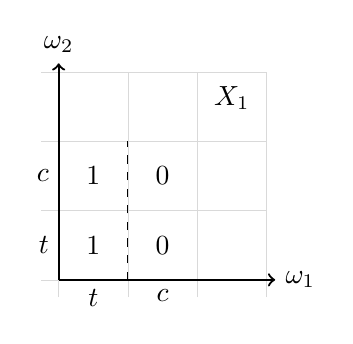
\begin{tikzpicture}[scale=1.1]
  \draw[step=0.8cm, gray!30, very thin] (-0.2,-0.2) grid (2.4,2.4);
  \draw[thick,->] (0,0)--(2.5,0) node[right]{$\omega_1$};
  \draw[thick,->] (0,0)--(0,2.5) node[above]{$\omega_2$};
  \node at (0.4,0.4){1};
  \node at (1.2,0.4){0};
  \node at (0.4,1.2){1};
  \node at (1.2,1.2){0};
  \node at (2,2.1){$\boldsymbol{X_1}$};
  \draw[dashed] (0.8,0)--(0.8,1.6);
  % etichette al centro delle celle
  \node[left] at (0,0.4){$t$};
  \node[left] at (0,1.2){$c$};
  \node[below] at (0.4,0){$t$};
  \node[below] at (1.2,0){$c$};
\end{tikzpicture}
\end{minipage}%
\hspace{0.5cm}
\begin{minipage}{0.4\textwidth}
\centering
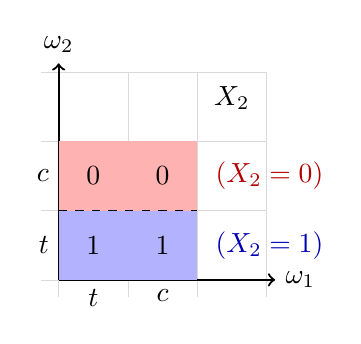
\begin{tikzpicture}[scale=1.1]
  \draw[step=0.8cm, gray!30, very thin] (-0.2,-0.2) grid (2.4,2.4);
  \draw[thick,->] (0,0)--(2.5,0) node[right]{$\omega_1$};
  \draw[thick,->] (0,0)--(0,2.5) node[above]{$\omega_2$};
  \fill[blue!30] (0,0) rectangle (1.6, 0.8);
  \fill[red!30] (0,0.8) rectangle (1.6,1.6);
  \node at (0.4,0.4){1};
  \node at (1.2,0.4){1};
  \node at (0.4,1.2){0};
  \node at (1.2,1.2){0};
  \node at (2,2.1){$\boldsymbol{X_2}$};
  \draw[dashed] (0,0.8)--(1.6,0.8);
  % etichette al centro
  \node[left] at (0,0.4){$t$};
  \node[left] at (0,1.2){$c$};
  \node[below] at (0.4,0){$t$};
  \node[below] at (1.2,0){$c$};
  \node[blue!70!black, right] at (1.7,0.4){$(X_2=1)$};
  \node[red!70!black, right] at (1.7,1.2){$(X_2=0)$};
\end{tikzpicture}
\end{minipage}%
\end{figure}

    Nel primo grafico si è sfruttato il fatto che il valore di $w_2$ non influisce in alcun modo su $X_1$; in modo del tutto analogo, per $X_2$ si è ragionato osservando che il suo valore non dipende da $w_1$.\\
    Siccome abbiamo già visto che $(X_1 +X_2)(w) := X_1(w) + X_2(w)$, allora ci basta sommare i valori per ogni $w$, riuscendo a trovare che la funzione somma si comporta come segue:
\begin{figure}[H]
\centering

\begin{minipage}{0.4\textwidth}
\centering
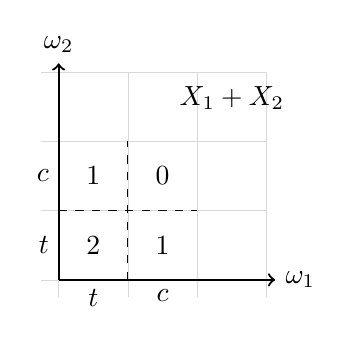
\begin{tikzpicture}[scale=1.1]
  \draw[step=0.8cm, gray!30, very thin] (-0.2,-0.2) grid (2.4,2.4);
  \draw[thick,->] (0,0)--(2.5,0) node[right]{$\omega_1$};
  \draw[thick,->] (0,0)--(0,2.5) node[above]{$\omega_2$};
  \node at (0.4,0.4){2};
  \node at (1.2,0.4){1};
  \node at (0.4,1.2){1};
  \node at (1.2,1.2){0};
  \node at (2,2.1){$\boldsymbol{X_1+X_2}$};
  \draw[dashed] (0.8,0)--(0.8,1.6);
  \draw[dashed] (0,0.8)--(1.6,0.8);
  % etichette al centro
  \node[left] at (0,0.4){$t$};
  \node[left] at (0,1.2){$c$};
  \node[below] at (0.4,0){$t$};
  \node[below] at (1.2,0){$c$};
\end{tikzpicture}
\end{minipage}%
\hspace{0cm}
\begin{minipage}{0.5\textwidth}
\centering
\[
\Rightarrow\qquad 
(X_1 + X_2)(\omega) =
\begin{cases}
    0, & \omega_1 = \omega_2 = c,\\[4pt]
    1, & \text{altrove},\\[4pt]
    2, & \omega_1 = \omega_2 = t.
\end{cases}
\]
\end{minipage}
\end{figure}

A questo punto possiamo andare a ragionare sulle controimmagini, per esempio:
\begin{itemize}
    \item \textcolor{red!70!black}{$(X_2 = 0)$}$ \:\overset{\text{def.}}{=} (w\in\Omega \mid X_2(w) = 0) = \set{(t, c), (c, c)}$
    \item \textcolor{blue!70!black}{$(X_1 = 0)$}$ \:\overset{\text{def.}}{=} (w\in\Omega \mid X_1(w) = 0) = \set{(t, t), (c, t)}$
    \item $(X_1 + X_2 = 1) = \set{(t, c), (c, c)}$
    \item $(X_1\leq\frac{1}{2}) = (X_1 = 0) = \set{(c, t), (c, c)}$
    \item $(X_1\leq\frac{1}{2}) \cup (X_2>0) = (X_1=0) \cup (X_2 = 1) = \set{(c, t), (c, c), (c, t)} = \left((X_1 = 1)\cap(X_2=0)\right)^c$
\end{itemize}
È importante notare di nuovo come la scrittura ``$(X_2=0)$'' vada letta come \textit{``gli elementi $w\in\Omega$ tali che l'applicazione di $X_2$ renda $0$''}. Stiamo quindi imponendo il valore della funzione a zero, e stiamo cercando quali elementi del dominio restituiscano $0$.\\
\\
Passiamo ora dalla notazione con $(t, c)$, a quella con $(1, 0)$, ed andiamo a considerare il caso di lanci ripetuti. Avremo quindi che:
\[\Omega = \set{0, 1}^\mathbb{N} = \set{(w_k)_{k\geq1}:w_k \in \{0, 1\}\;\forall k\geq1}\]
$\Omega$ risulta quindi essere equipollente ad $\mathbb{N}$ (e quindi non numerabile), composto dalle successioni di $(0, 1)$. Introduciamo ora: 
\[X_n(\ve{w}) = w_n\]
dove $\ve{w}$ rappresenta una singola successione (come vettore), e la funzione restituisce l'ennesimo valore di quest'ultima\footnote{Per esempio: $\ve{w} = (1, 0, 0, 1, 1, 0, ...)\Rightarrow X_4(\ve{w}) = 1$}. \\
Quindi, $\forall n\geq1: \quad X_n:\Omega\to\{0, 1\}$\\
\\Allora si avrà per esempio che:
\begin{itemize}
    \item $(X_2 = 0) = \{w\in\{0, 1\}\mathbb{N}: \; w_2 = 0\}$
    \item $(X_1X_2 = 0) =\{w\in\{0, 1\}^\mathbb{N}:\;w_1=0 \text{ oppure } w_2 = 0\} = \{w\in\{0, 1\}^\mathbb{N}:\; w_1=w_2=1\}^c$ 
    \item Se volessimo modellizzare l'evento ``non esce mai croce'': \\
    $\bigcap_{n=1}^\infty (X_n = 1 ) = \set{1, 1, 1, ..., 1, 1, ...}$
\end{itemize}
\end{esempio}